
%% bare_conf.tex
%% V1.3
%% 2007/01/11
%% by Michael Shell
%% See:
%% http://www.michaelshell.org/
%% for current contact information.
%%
%% This is a skeleton file demonstrating the use of IEEEtran.cls
%% (requires IEEEtran.cls version 1.7 or later) with an IEEE conference paper.
%%
%% Support sites:
%% http://www.michaelshell.org/tex/ieeetran/
%% http://www.ctan.org/tex-archive/macros/latex/contrib/IEEEtran/
%% and
%% http://www.ieee.org/

%%*************************************************************************
%% Legal Notice:
%% This code is offered as-is without any warranty either expressed or
%% implied; without even the implied warranty of MERCHANTABILITY or
%% FITNESS FOR A PARTICULAR PURPOSE!
%% User assumes all risk.
%% In no event shall IEEE or any contributor to this code be liable for
%% any damages or losses, including, but not limited to, incidental,
%% consequential, or any other damages, resulting from the use or misuse
%% of any information contained here.
%%
%% All comments are the opinions of their respective authors and are not
%% necessarily endorsed by the IEEE.
%%
%% This work is distributed under the LaTeX Project Public License (LPPL)
%% ( http://www.latex-project.org/ ) version 1.3, and may be freely used,
%% distributed and modified. A copy of the LPPL, version 1.3, is included
%% in the base LaTeX documentation of all distributions of LaTeX released
%% 2003/12/01 or later.
%% Retain all contribution notices and credits.
%% ** Modified files should be clearly indicated as such, including  **
%% ** renaming them and changing author support contact information. **
%%
%% File list of work: IEEEtran.cls, IEEEtran_HOWTO.pdf, bare_adv.tex,
%%                    bare_conf.tex, bare_jrnl.tex, bare_jrnl_compsoc.tex
%%*************************************************************************

% *** Authors should verify (and, if needed, correct) their LaTeX system  ***
% *** with the testflow diagnostic prior to trusting their LaTeX platform ***
% *** with production work. IEEE's font choices can trigger bugs that do  ***
% *** not appear when using other class files.                            ***
% The testflow support page is at:
% http://www.michaelshell.org/tex/testflow/



% Note that the a4paper option is mainly intended so that authors in
% countries using A4 can easily print to A4 and see how their papers will
% look in print - the typesetting of the document will not typically be
% affected with changes in paper size (but the bottom and side margins will).
% Use the testflow package mentioned above to verify correct handling of
% both paper sizes by the user's LaTeX system.
%
% Also note that the "draftcls" or "draftclsnofoot", not "draft", option
% should be used if it is desired that the figures are to be displayed in
% draft mode.
%

\documentclass[conference]{IEEEtran}
% Add the compsoc option for Computer Society conferences.
%
% If IEEEtran.cls has not been installed into the LaTeX system files,
% manually specify the path to it like:
% \documentclass[conference]{../sty/IEEEtran}





% Some very useful LaTeX packages include:
% (uncomment the ones you want to load)


% *** MISC UTILITY PACKAGES ***
%
%\usepackage{ifpdf}
% Heiko Oberdiek's ifpdf.sty is very useful if you need conditional
% compilation based on whether the output is pdf or dvi.
% usage:
% \ifpdf
%   % pdf code
% \else
%   % dvi code
% \fi
% The latest version of ifpdf.sty can be obtained from:
% http://www.ctan.org/tex-archive/macros/latex/contrib/oberdiek/
% Also, note that IEEEtran.cls V1.7 and later provides a builtin
% \ifCLASSINFOpdf conditional that works the same way.
% When switching from latex to pdflatex and vice-versa, the compiler may
% have to be run twice to clear warning/error messages.

% *** CITATION PACKAGES ***
%
%\usepackage{cite}
% cite.sty was written by Donald Arseneau
% V1.6 and later of IEEEtran pre-defines the format of the cite.sty package
% \cite{} output to follow that of IEEE. Loading the cite package will
% result in citation numbers being automatically sorted and properly
% "compressed/ranged". e.g., [1], [9], [2], [7], [5], [6] without using
% cite.sty will become [1], [2], [5]--[7], [9] using cite.sty. cite.sty's
% \cite will automatically add leading space, if needed. Use cite.sty's
% noadjust option (cite.sty V3.8 and later) if you want to turn this off.
% cite.sty is already installed on most LaTeX systems. Be sure and use
% version 4.0 (2003-05-27) and later if using hyperref.sty. cite.sty does
% not currently provide for hyperlinked citations.
% The latest version can be obtained at:
% http://www.ctan.org/tex-archive/macros/latex/contrib/cite/
% The documentation is contained in the cite.sty file itself.


%\usepackage{program}
\newtheorem{algorithm}{Algorithm}
\usepackage{algpseudocode}
\usepackage{varwidth}
\usepackage{graphicx}
\graphicspath{{./images}}
\usepackage{hyperref}
\hypersetup{colorlinks=true}


%\usepackage[]{algorithm2e}


% *** GRAPHICS RELATED PACKAGES ***
% \ifCLASSINFOpdf
%   % \usepackage[pdftex]{graphicx}
%   % declare the path(s) where your graphic files are
%   % \graphicspath{{../pdf/}{../jpeg/}}
%   % and their extensions so you won't have to specify these with
%   % every instance of \includegraphics
%   % \DeclareGraphicsExtensions{.pdf,.jpeg,.png}
% \else
%   % or other class option (dvipsone, dvipdf, if not using dvips). graphicx
%   % will default to the driver specified in the system graphics.cfg if no
%   % driver is specified.
%   % \usepackage[dvips]{graphicx}
%   % declare the path(s) where your graphic files are
%   % \graphicspath{{../eps/}}
%   % and their extensions so you won't have to specify these with
%   % every instance of \includegraphics
%   % \DeclareGraphicsExtensions{.eps}
% \fi
% graphicx was written by David Carlisle and Sebastian Rahtz. It is
% required if you want graphics, photos, etc. graphicx.sty is already
% installed on most LaTeX systems. The latest version and documentation can
% be obtained at:
% http://www.ctan.org/tex-archive/macros/latex/required/graphics/
% Another good source of documentation is "Using Imported Graphics in
% LaTeX2e" by Keith Reckdahl which can be found as epslatex.ps or
% epslatex.pdf at: http://www.ctan.org/tex-archive/info/
%
% latex, and pdflatex in dvi mode, support graphics in encapsulated
% postscript (.eps) format. pdflatex in pdf mode supports graphics
% in .pdf, .jpeg, .png and .mps (metapost) formats. Users should ensure
% that all non-photo figures use a vector format (.eps, .pdf, .mps) and
% not a bitmapped formats (.jpeg, .png). IEEE frowns on bitmapped formats
% which can result in "jaggedy"/blurry rendering of lines and letters as
% well as large increases in file sizes.
%
% You can find documentation about the pdfTeX application at:
% http://www.tug.org/applications/pdftex


% *** MATH PACKAGES ***
%
\usepackage[cmex10]{amsmath}
% A popular package from the American Mathematical Society that provides
% many useful and powerful commands for dealing with mathematics. If using
% it, be sure to load this package with the cmex10 option to ensure that
% only type 1 fonts will utilized at all point sizes. Without this option,
% it is possible that some math symbols, particularly those within
% footnotes, will be rendered in bitmap form which will result in a
% document that can not be IEEE Xplore compliant!
%
% Also, note that the amsmath package sets \interdisplaylinepenalty to 10000
% thus preventing page breaks from occurring within multiline equations. Use:
%\interdisplaylinepenalty=2500
% after loading amsmath to restore such page breaks as IEEEtran.cls normally
% does. amsmath.sty is already installed on most LaTeX systems. The latest
% version and documentation can be obtained at:
% http://www.ctan.org/tex-archive/macros/latex/required/amslatex/math/


% *** SPECIALIZED LIST PACKAGES ***
%
%\usepackage{algorithmic}
% algorithmic.sty was written by Peter Williams and Rogerio Brito.
% This package provides an algorithmic environment fo describing algorithms.
% You can use the algorithmic environment in-text or within a figure
% environment to provide for a floating algorithm. Do NOT use the algorithm
% floating environment provided by algorithm.sty (by the same authors) or
% algorithm2e.sty (by Christophe Fiorio) as IEEE does not use dedicated
% algorithm float types and packages that provide these will not provide
% correct IEEE style captions. The latest version and documentation of
% algorithmic.sty can be obtained at:
% http://www.ctan.org/tex-archive/macros/latex/contrib/algorithms/
% There is also a support site at:
% http://algorithms.berlios.de/index.html
% Also of interest may be the (relatively newer and more customizable)
% algorithmicx.sty package by Szasz Janos:
% http://www.ctan.org/tex-archive/macros/latex/contrib/algorithmicx/

% *** ALIGNMENT PACKAGES ***
%
%\usepackage{array}
% Frank Mittelbach's and David Carlisle's array.sty patches and improves
% the standard LaTeX2e array and tabular environments to provide better
% appearance and additional user controls. As the default LaTeX2e table
% generation code is lacking to the point of almost being broken with
% respect to the quality of the end results, all users are strongly
% advised to use an enhanced (at the very least that provided by array.sty)
% set of table tools. array.sty is already installed on most systems. The
% latest version and documentation can be obtained at:
% http://www.ctan.org/tex-archive/macros/latex/required/tools/


%\usepackage{mdwmath}
%\usepackage{mdwtab}
% Also highly recommended is Mark Wooding's extremely powerful MDW tools,
% especially mdwmath.sty and mdwtab.sty which are used to format equations
% and tables, respectively. The MDWtools set is already installed on most
% LaTeX systems. The lastest version and documentation is available at:
% http://www.ctan.org/tex-archive/macros/latex/contrib/mdwtools/


% IEEEtran contains the IEEEeqnarray family of commands that can be used to
% generate multiline equations as well as matrices, tables, etc., of high
% quality.


%\usepackage{eqparbox}
% Also of notable interest is Scott Pakin's eqparbox package for creating
% (automatically sized) equal width boxes - aka "natural width parboxes".
% Available at:
% http://www.ctan.org/tex-archive/macros/latex/contrib/eqparbox/

% *** SUBFIGURE PACKAGES ***
%\usepackage[tight,footnotesize]{subfigure}
% subfigure.sty was written by Steven Douglas Cochran. This package makes it
% easy to put subfigures in your figures. e.g., "Figure 1a and 1b". For IEEE
% work, it is a good idea to load it with the tight package option to reduce
% the amount of white space around the subfigures. subfigure.sty is already
% installed on most LaTeX systems. The latest version and documentation can
% be obtained at:
% http://www.ctan.org/tex-archive/obsolete/macros/latex/contrib/subfigure/
% subfigure.sty has been superceeded by subfig.sty.



%\usepackage[caption=false]{caption}
%\usepackage[font=footnotesize]{subfig}
% subfig.sty, also written by Steven Douglas Cochran, is the modern
% replacement for subfigure.sty. However, subfig.sty requires and
% automatically loads Axel Sommerfeldt's caption.sty which will override
% IEEEtran.cls handling of captions and this will result in nonIEEE style
% figure/table captions. To prevent this problem, be sure and preload
% caption.sty with its "caption=false" package option. This is will preserve
% IEEEtran.cls handing of captions. Version 1.3 (2005/06/28) and later
% (recommended due to many improvements over 1.2) of subfig.sty supports
% the caption=false option directly:
%\usepackage[caption=false,font=footnotesize]{subfig}
%
% The latest version and documentation can be obtained at:
% http://www.ctan.org/tex-archive/macros/latex/contrib/subfig/
% The latest version and documentation of caption.sty can be obtained at:
% http://www.ctan.org/tex-archive/macros/latex/contrib/caption/

% *** FLOAT PACKAGES ***
%
%\usepackage{fixltx2e}
% fixltx2e, the successor to the earlier fix2col.sty, was written by
% Frank Mittelbach and David Carlisle. This package corrects a few problems
% in the LaTeX2e kernel, the most notable of which is that in current
% LaTeX2e releases, the ordering of single and double column floats is not
% guaranteed to be preserved. Thus, an unpatched LaTeX2e can allow a
% single column figure to be placed prior to an earlier double column
% figure. The latest version and documentation can be found at:
% http://www.ctan.org/tex-archive/macros/latex/base/

%\usepackage{stfloats}
% stfloats.sty was written by Sigitas Tolusis. This package gives LaTeX2e
% the ability to do double column floats at the bottom of the page as well
% as the top. (e.g., "\begin{figure*}[!b]" is not normally possible in
% LaTeX2e). It also provides a command:
%\fnbelowfloat
% to enable the placement of footnotes below bottom floats (the standard
% LaTeX2e kernel puts them above bottom floats). This is an invasive package
% which rewrites many portions of the LaTeX2e float routines. It may not work
% with other packages that modify the LaTeX2e float routines. The latest
% version and documentation can be obtained at:
% http://www.ctan.org/tex-archive/macros/latex/contrib/sttools/
% Documentation is contained in the stfloats.sty comments as well as in the
% presfull.pdf file. Do not use the stfloats baselinefloat ability as IEEE
% does not allow \baselineskip to stretch. Authors submitting work to the
% IEEE should note that IEEE rarely uses double column equations and
% that authors should try to avoid such use. Do not be tempted to use the
% cuted.sty or midfloat.sty packages (also by Sigitas Tolusis) as IEEE does
% not format its papers in such ways.

% *** PDF, URL AND HYPERLINK PACKAGES ***
%
%\usepackage{url}
% url.sty was written by Donald Arseneau. It provides better support for
% handling and breaking URLs. url.sty is already installed on most LaTeX
% systems. The latest version can be obtained at:
% http://www.ctan.org/tex-archive/macros/latex/contrib/misc/
% Read the url.sty source comments for usage information. Basically,
% \url{my_url_here}.

% *** Do not adjust lengths that control margins, column widths, etc. ***
% *** Do not use packages that alter fonts (such as pslatex).         ***
% There should be no need to do such things with IEEEtran.cls V1.6 and later.
% (Unless specifically asked to do so by the journal or conference you plan
% to submit to, of course. )


% correct bad hyphenation here
% \hyphenation{op-tical net-works semi-conduc-tor}

% paper title
% can use linebreaks \\ within to get better formatting as desired
\title{Leveraging Input Space Sparsity\\ to Scale Tree-Based Models}

% author names and affiliations
% use a multiple column layout for up to three different
% affiliations
\author{
\IEEEauthorblockN{Fares Hedayati}
\IEEEauthorblockA{Elance-oDesk\\
                  Dept. of Data Science\\
                  441 Logue Ave, Mountain View, CA 94043\\
                  Email: fares19@elance-odesk.com}
\and
\IEEEauthorblockN{Arnaud Joly}
\IEEEauthorblockA{Dept. of EE \& CS \& GIGA-R\\
                  University of Li�ge\\
                  Belgium\\
                  Email: a.joly@ulg.ac.be
}
\and
\IEEEauthorblockN{Panagiotis Papadimitriou}
\IEEEauthorblockA{Elance-oDesk\\
                  Dept. of Data Science\\
                  441 Logue Ave, Mountain View, CA 94043\\
                  Email: papadimitriou@elance-odesk.com}
}

% conference papers do not typically use \thanks and this command
% is locked out in conference mode. If really needed, such as for
% the acknowledgment of grants, issue a \IEEEoverridecommandlockouts
% after \documentclass

% for over three affiliations, or if they all won't fit within the width
% of the page, use this alternative format:
%
%\author{\IEEEauthorblockN{Michael Shell\IEEEauthorrefmark{1},
%Homer Simpson\IEEEauthorrefmark{2},
%James Kirk\IEEEauthorrefmark{3},
%Montgomery Scott\IEEEauthorrefmark{3} and
%Eldon Tyrell\IEEEauthorrefmark{4}}
%\IEEEauthorblockA{\IEEEauthorrefmark{1}School of Electrical and Computer Engineering\\
%Georgia Institute of Technology,
%Atlanta, Georgia 30332--0250\\ Email: see http://www.michaelshell.org/contact.html}
%\IEEEauthorblockA{\IEEEauthorrefmark{2}Twentieth Century Fox, Springfield, USA\\
%Email: homer@thesimpsons.com}
%\IEEEauthorblockA{\IEEEauthorrefmark{3}Starfleet Academy, San Francisco, California 96678-2391\\
%Telephone: (800) 555--1212, Fax: (888) 555--1212}
%\IEEEauthorblockA{\IEEEauthorrefmark{4}Tyrell Inc., 123 Replicant Street, Los Angeles, California 90210--4321}}

% use for special paper notices
%\IEEEspecialpapernotice{(Invited Paper)}

% make the title area
\begin{document}
\maketitle

\begin{abstract}

Many machine learning tasks such as text annotation involve sparsely
representable input space. State-of-the-art tree-based ensemble algorithms and
implementations have focused on tasks with dense input space, while at most
emulating random memory access on sparse input data. We propose a fast and an
efficient splitting algorithm to leverage input sparsity within decision tree
methods. We exploit the a-priori knowledge that each column have very few non-
zero elements and show how learning time is significantly decreased.

\end{abstract}
% IEEEtran.cls defaults to using nonbold math in the Abstract.
% This preserves the distinction between vectors and scalars. However,
% if the conference you are submitting to favors bold math in the abstract,
% then you can use LaTeX's standard command \boldmath at the very start
% of the abstract to achieve this. Many IEEE journals/conferences frown on
% math in the abstract anyway.

% no keywords

% For peer review papers, you can put extra information on the cover
% page as needed:
% \ifCLASSOPTIONpeerreview
% \begin{center} \bfseries EDICS Category: 3-BBND \end{center}
% \fi
%
% For peerreview papers, this IEEEtran command inserts a page break and
% creates the second title. It will be ignored for other modes.
\IEEEpeerreviewmaketitle

\section{Introduction}
% no \IEEEPARstart

High dimensional supervised learning problems, e.g. in text or image
annotation, are more frequent than ever. It consists in searching a mapping
between an input space, where each dimension is called a feature
to some  categorical or numerical output variable. A sample is a
input-output pair. While those datasets have very high dimensional input space,
they are often sparsely representable. For instance, the number of unique words
associated to a text document is actually small compared to the all words of a
given language. In order to work efficiently with such data, efficient matrix
formats have been developed with fast operations, such as dot product, and a
low memory footprints.

Tree-based ensemble models, such as adaboost \cite{freund1995desicion}, random
forest \cite{breiman2001random} or gradient tree boosting
\cite{friedman2001greedy}, are some of the most robust and widely-used
supervised machine learning. All these methods have in common that they use
randomized decision trees as a base learner. This building block is a
hierarchical model which divide the input space through a serie of binary
splitting rules which partition the input space . Predictions of a decision tree is obtained by
following the tree structure until reaching a leaf. In the ensemble framework, those models are either averaged
\cite{breiman2001random} or learnt sequentially \cite{freund1995desicion},
\cite{friedman2001greedy}.

Many models, such as linear or nearest neighbors model, could directly benefit
from the input sparsity by formulating the entire algorithm through a set of
dot products. However this is not possible for tree based methods, most machine
learning packages don't support sparse input for tree-based methods, are
restricted to decision stumps (decision tree with only one internal node) or
have a sub-optimal implementation through the simulation of a random access
memory as in the dense case. The only solution is often to densify the input
space which leads first to severe memory constraints and then to slow
training time.

In this paper, we present an efficient splitting procedure tailored for
numerical sparse input data in compressed sparse column format, a sparse matrix
format. For a given subset of samples, we are able to efficiently extract non
zero values for a given feature of this subset of samples. Knowing which
elements are non zeros allows large speed up. It decreases sorting time of
samples in the current node along features which is an essential component in
all tree-based models. Moreover it reduces the set of possible splits to
evaluate at each node. We also want to highlight that the contribution of this
paper have been proposed for inclusion to the  \emph{scikit-learn}
\cite{buitinck2013api,pedregosa2011scikit} open source package. This will
benefit the machine learning community.

The rest of this paper is organized as follows: Section \ref{sec:background}
introduces decision tree splitting algorithm and sparse matrix formats; Section
\ref{sec:sparse-input-dt} describes the proposed splitting algorithm for sparse
input data; Section \ref{sec:experiments} provides our empirical implementation
study and Section \ref{sec:conclusion} concludes and describes further
perspectives.

\section{Background} \label{sec:background}
\subsection{Induction of decision trees}

We denote by $\mathcal{X}$ an input space and by $\mathcal{Y}$ the output space.
Without loss of generality, we suppose that $\mathcal{X} = \mathcal{R}^p$ where
$p$ denotes the number of features. Learning samples are represented by a pair of matrix
$(X, Y) \subseteq (\mathcal{X}, \mathcal{Y})_{i=0}^{n-1}$, where each row
corresponds to a sample and each column to a feature or an output variable.

A decision trees \cite{breiman1984classification} is built  by recursively
maximizing the average reduction of an impurity measure, such as the variance,
\[
\Delta{}I(s, \mathcal{L}) =
I((Y_i)_{i�\in \mathcal{L}}) -
\frac{|\mathcal{L}_r|}{|\mathcal{L}|} I((Y_i)_{i�\in \mathcal{L}_l}) -
\frac{|\mathcal{L}_l|}{|\mathcal{L}|} I((Y_i)_{i�\in \mathcal{L}_r}))
\]
where $s$ is a binary partition of the input space which divide the sample set
$\mathcal{L}$ into $ \mathcal{L}_l$ and $ \mathcal{L}_r$. This recursive
procedure is repeated until a stopping condition is met, e.g. a maximal depth
is reached or there are too few samples to split. Those stopping criteria act
as regularization parameters. Leaves are labeled by the output mean in
regression or by the class frequencies in classification with reaching training
samples. The recursive induction of the decision decision is described
by Algorithm~\ref{algo:tree-induction} and the search for the best split
is described by  Algorithm~\ref{algo:find-best-split}.

In the context of ensemble, tree are further randomized by searching for the
best split among $k$ features at each node and also might be induced on a
bootstrap copy of the samples. The tree can be grown alternatively in a best-first
search manner by replacing the stack of Algorithm~\ref{algo:tree-induction}
by a priority queue where priority is defined by expected impurity reduction.

\begin{algorithm}\label{algo:tree-induction}
Build a decision tree
\textnormal{
\begin{algorithmic}[1]
\Function{InduceDecisionTree}{$X$, $Y$}
    \State Initialize a tree structure $\tau$ with root node $t_0$
    \State Initialize an empty stack $stack$
    \State Initialize a sample set $\mathcal{L}=\{0,\ldots,n-1\}$
    \State $stack$\Call{.push}{($t_0$, $\mathcal{L}$)}
    \While{$stack$ is not empty}
        \State $t_p$, $\mathcal{L}_p$ = $stack$\Call{.pop}{}()
        \If{$t_p$ satisfies stopping criterion}
            \State Make $t_p$ a leaf node using $\mathcal{L}_p$ and $Y$.
        \Else
            \State \begin{varwidth}[t]{0.8\linewidth}
                   Find a splitting rule $s^*$ which maximizes impurity reduction
                   among possible splitting rules $Q(\mathcal{L}_p, X)$:
                   \[
                   s^* = \arg\max_{s \in Q(\mathcal{L}_p, X)} \Delta{}I(s, \mathcal{L}_p).
                   \]
                   \end{varwidth}
            \State Make $t_p$ an internal node given splitting rule $s$.
            \State Partition $\mathcal{L}_p$ into $\mathcal{L}_r$ and
                   $\mathcal{L}_l$ given $s^*$. \label{alg-line:partition}
            \State Create two empty nodes $t_r$ and $t_l$ child of $t_p$.
            \State $stack$\Call{.push}{($t_r$, $\mathcal{L}_r$)}
            \State $stack$\Call{.push}{($t_l$, $\mathcal{L}_l$)}
        \EndIf
    \EndWhile
    \State \Return $\tau$
\EndFunction
\end{algorithmic}
}
\end{algorithm}

\begin{algorithm}\label{algo:find-best-split}
Search for the best split
\textnormal{
\begin{algorithmic}[1]
\Function{FindBestSplit}{$\mathcal{L}$, $X$, $Y$}
    \State $\text{best} = -\infty$
    \For{$j \in \{0, \ldots, p-1\}$}
        \State Extract feature values reaching the node
               \[
               \mathcal{X}_j = \{X_{i,j}, \forall i \in \mathcal{L}\}.
               \] \label{alg-line:value-extract}
        \State Sort $\mathcal{L}$ and $\mathcal{X}_j$ by increasing values
               of $\mathcal{X}_j$.  \label{alg-line:sorting}
        \State Generate all possible splitting rules
               \[
               Q(\mathcal{X}_j)=\{((x_j \leq \nu), (x_j > \nu))| \nu�\in�\mathcal{X}_j)
               \]
        \For{$s$ in $Q(\mathcal{X}_j)$}
            \State Evaluate impurity reduction of splitting rule $s$
                   \[
                   \text{score} = \Delta{}I(s, \mathcal{L}).
                   \]
            \If{$\text{score} > \text{best}$}
                \State $\text{best} =\text{score}$
                \State $s^* = s$
            \EndIf
        \EndFor
    \EndFor
    \State \Return $s^*$
\EndFunction
\end{algorithmic}
}
\end{algorithm}

\subsection{Sparse matrix format}

For memory efficiency and taking advantage of sparsity we use a data structure
called compressed sparse column (csc) matrix format. It is a general format to
represent compactly sparse matrices using three arrays: a $data$ array stores
the value of each non zero elements, an $indices$ array stores the row index
of each non zero elements and an $indptr$ array which stores the beginning and
end of each columns in the $data$ and the $indices$ arrays.

For instance, this $3 \times 5$ matrix
\[
\begin{bmatrix}
1 & 0 & 0 & 4 & 0 \\
0 & 0 & 0 & 5 & 0 \\
0 & 0 & 0 & 0 & 0
\end{bmatrix}
\]
is represented by the following csc matrix with arrays
\begin{align*}
inptr &= \begin{bmatrix}0 & 1 & 1 & 1 & 3 & 3\end{bmatrix}, \\
indices &= \begin{bmatrix}0 & 0 & 1\end{bmatrix},�\\
data &= \begin{bmatrix}1 & 4 & 5\end{bmatrix}.
\end{align*}

The main advantages of csc matrices are to allow fast column indexing, efficient
arithmetic and matrix operations. However, row indexing is slow. Note that a
similar row-based sparse matrix called compressed sparse row format also exists
and works under similar principles.

\section{Growth of decision trees on sparse input data} \label{sec:sparse-input-dt}

In order to grow decision trees on sparse input matrix, we have to require a
sparse matrix format with efficient row indexing as the tree works with subset
of the samples, and also efficient column indexing as features are randomly
sampled at each node. Furthermore, we hope to speed up the overall algorithm by
taking into account the input space sparsity. Compressed sparse column matrix
already satisfies the fast column indexing requirement. We are going to show
how to efficiently exploit the data structure as to have a fast row indexing
and use the proposed approach to speed up the overall algorithm on sparse data.

Given the sparse matrix format, the main issue is to efficiently perform the
extraction of the sample values reaching the node (the line \ref{alg-line:value-extract}
of Algorithm \ref{algo:find-best-split}). Note that this is the only operation which requires interaction
with the input matrix data. Otherwise said for a
given feature $j$, one have to be able to perform the intersection between the
sample set $\mathcal{L}_p$ which have reached the node and the $m_j=indptr[j+1] -
indptr[j]$  non zero elements of the feature $j$ as to generate a set of
possible splitting rules. If we assume that the $indices$ of the input csc matrix
array are sorted per column, then standard intersection
algorithms have the following time complexity:
\begin{enumerate}
\item in $O(|\mathcal{L}_p| \log{m_j})$ by performing $|\mathcal{L}_p| $ binary
search on the sorted $m_j$ non zero elements;
\item in $O(|\mathcal{L}_p|\log{|\mathcal{L}_p|} + m_j\log{|\mathcal{L}_p|})$
by sorting the sample set $\mathcal{L}$ and performing $m_j$ binary search on
$\mathcal{L}_p$;
\item in $O(|\mathcal{L}_p|\log{|\mathcal{L}_p|} + m_j + |\mathcal{L}_p|)$ by sorting the
sample set $\mathcal{L}_p$ and retrieving the intersection by iterating over both
arrays;
\item in $O(m_j + |\mathcal{L}_p|)$ by first creating a temporary hash table from the
a first array and then checking if elements of the second array are contained
in the hash table.
\end{enumerate}

In the context of decision tree induction, the intersection operation will be
repeated for each sampled feature and for various sample sets $\mathcal{L}_p$.
Taking this into account, it's possible to improve approach (4). The idea is to
maintain during the tree growth a mapping, represented at Figure
\ref{fig:mapping}, between the row index, the $indices$ array, of the csc
matrix and the position of the related samples in the sample set array
$\mathcal{L}$. Since each sample only belongs to one tree branch, a subset
$\mathcal{L}_p$ of $\mathcal{L}$ can be conveniently represented by a slice
$[start, end[$ of the array $\mathcal{L}$. Thus, it's possible to check in
$O(1)$ if the $k$-th non zero element of the csc matrix belongs to the sample set
$\mathcal{L}_p$ by checking if $mapping[indices[k]]$ is in $[start, end[$.
Maintaining the mapping for a given position $p$ is done in $O(1)$ by
setting $mapping[\mathcal{L}[p]]$ to $p$. Thus we deduce that performing
the intersection between the $indices$ array and $\mathcal{L}_p$ can be
done in $O(m_j)$.

\begin{figure}
  \centering
   \def\svgwidth{0.4\textwidth}
   \input{images/mapping.pdf_tex}
   \caption{The array $mapping$ allow to efficiently know if between the $indices$ array of the csr matrix
            and a sample set $\mathcal{L}_p$}
   \label{fig:mapping}
\end{figure}

With the application of the mapping intersection algorithm, we can speed up the
sorting operation and splitting rule evaluation of Algorithm~\ref{algo:find-best-split}
by working separately on positive and negative values. Furthermore, it's also
possible to partition a
sample set $\mathcal{L}_p$ into two partition $\mathcal{L}_r$ and
$\mathcal{L}_r$ (line~ \ref{alg-line:partition} of Algorithm~\ref{algo:tree-induction})
given a split on feature $j$ in $O(m_j)$ instead of $O(n)$.

In practice, the number of non zero elements $m_j$ of feature $j$ could be a
lot bigger than the size of a sample set $\mathcal{L}_p$. This is likely to
happen near the leaf nodes. Whenever the tree is fully developed, there are
only a few   samples reaching those nodes. For optimal performance, one can use
a hybrid intersection approach which combines the previously developed mapping
intersection to approach (1) based on binary search. whenever $\mathcal{L}_p \ll
m_j$, the binary approach will be faster.

During the tree growth, one could remember which features are constant for a
subset of the samples $\mathcal{L}_p$ and a given node $t_p$. For all
descendant of node $t_p$, this will avoid the overhead of searching for a best
split where none exists.

Finally note that for testing the sparse data is flattened for efficient random
memory access.

\section{Experiments} \label{sec:experiments}

In the first experiment we trained different decision tree classifiers on the \emph{20 Newsgroups} dataset, changing the $max\_depth$ only and keeping the default values for others, i.e. $min\_samples\_split=2$ and $min\_samples\_leaf=1$. The dataset
consists of $20000$ news groups documents distributed across $20$ newsgroups
almost evenly \cite{joachims1996probabilistic}. For each value of $max\_depth$ we trained two decision tree classifiers: one time with the training data represented in a $csc\_matrix$ sparse matrix and one time with the data represented in a dense matrix. For each of these pairs we verified that the trees are identical and compared their training times. As Figure~\ref{depth} shows, the training time with a densely represented matrix is much higher than its sparsely represented counterpart.

\begin{figure}[h]
\centering
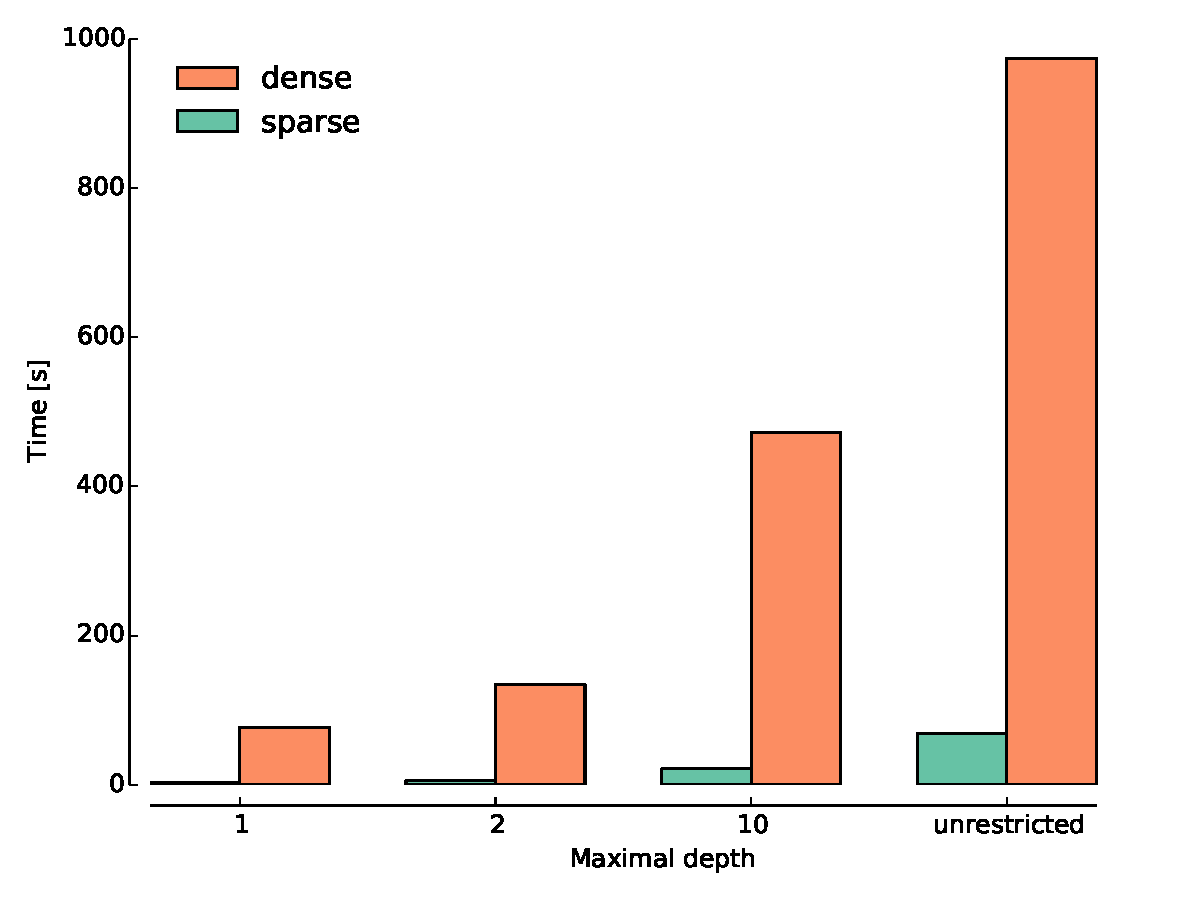
\includegraphics[scale=0.45]{images/depth.pdf}%20_news_groups.png
\caption{Training Time for Different $max\_depth$ on Sparse vs. Dense Input
         (20 News Groups)}
\label{depth}
\end{figure}

The second experiment was carried out on synthetic data. This time we trained different decision tree classifiers, with $max\_depth = 20$ and keeping the default values for other parameters. We generated random matrices of varying densities
each of size $100000 \times 1000$. Density is the percentage
of non-zero values for each feature. For example in a matrix with $density=0.1$ every feature is $10\%$ of the time non-zero. For each density we created $10$ random matrices, and each of these matrices were represented in a sparse $csc\_matrix$ and a dense matrix and decision tree classifiers were fitted on both formats. Figure~\ref{density} shows the average training time for each density with one standard deviation. As the figure shows the training time of sparse matrices is much lower that their dense
counterparts when the density of the matrix is quite low, i.e. less than $0.2$. On the other hand when the density is high, e.g. $density = 0.5$, the training time with dense matrices
input is lower than their sparse counterparts. The figure suggests that $csc\_matrix$ should only be used when the data is really sparse, e.g. with textual data.


\begin{figure}[h]
\centering
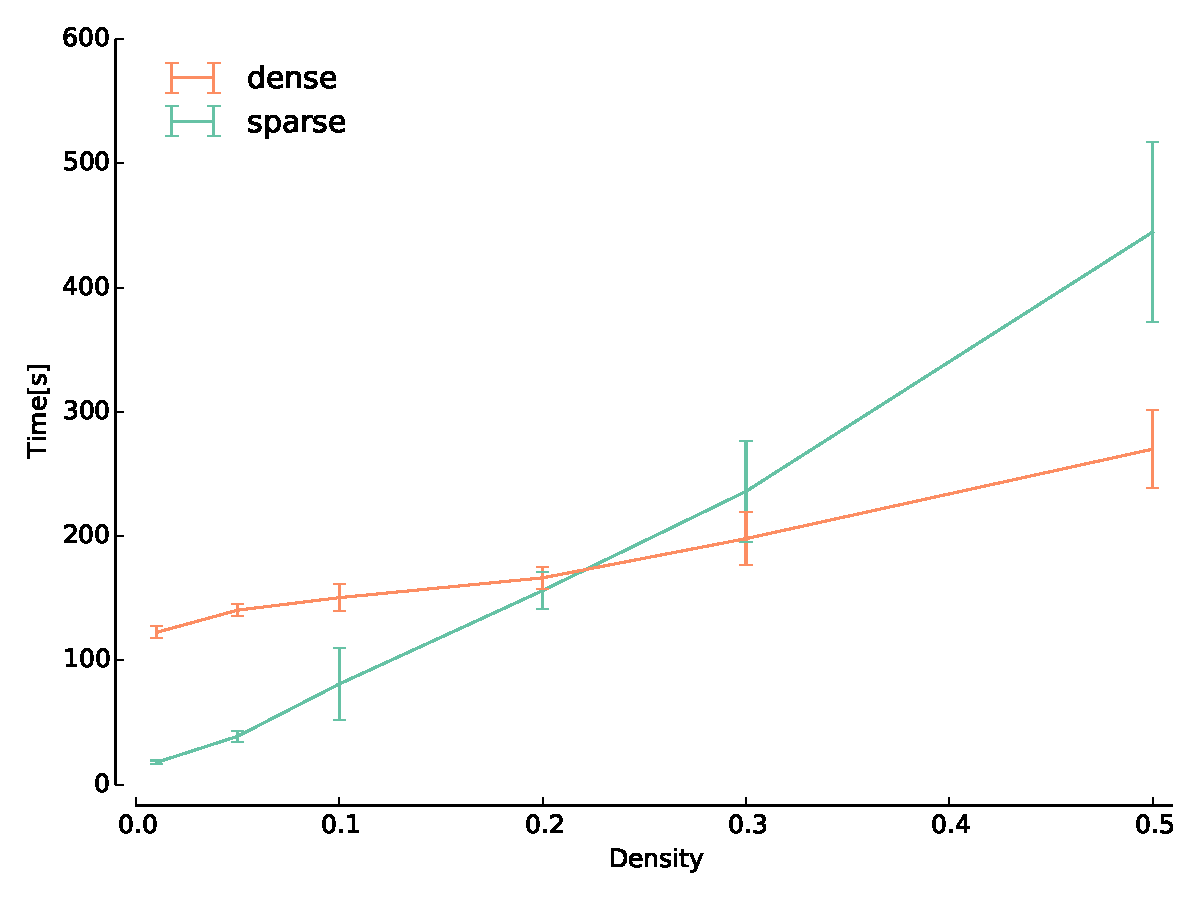
\includegraphics[scale=0.45]{images/density.pdf}
\caption{Training Time of Random Matrices with $n\_samples = 100000$, $n\_features = 1000$ and Different Densities on Sparse vs. Dense Input}
\label{density}
\end{figure}

%\begin{table}[h]
%\caption {Training Time in Seconds with Sparse and Dense Inputs} \label{density}
%\begin{tabular}{|l|l|l||l|l|l|}
%  \hline
%Dataset Size	&	Feature Size	&	density	&	 Sparse Input	&	Dense Input	\\
%  \hline
%10000	  &	1000	&	0.01	&	4.74	&	25.07	\\
%100000	&	100	&	0.01	&	7.26	&	24.65	\\
%100000	&	1000	&	0.01	&	89.13	&	507.86	\\
%10000	  &	1000	&	0.05	&	9.82	&	16.14	\\
%100000	&	100	&	0.05	&	21.14	&	28.27	\\
%100000	&	1000	&	0.05	&	256.68	&	541.00	\\
%10000	  &	1000	&	0.1	&	13.42	&	12.38	\\
%100000 	&	100	&	0.1	&	37.81	&	24.65	\\
%100000	&	1000	&	0.1	&	437.14	&	370.60	\\
%10000	  &	1000	&	0.5	&	28.97	&	14.02	\\
%100000	&	100	&	0.5	&	100.22	&	28.13	\\
%100000	&	1000	&	0.5	&	949.14	&	383.62 \\
% \hline
%\end{tabular}
%\end{table}

\section{Conclusion}\label{sec:conclusion}
The conclusion goes here.

\section*{Acknowledgment} % use section* for acknowledgement

Arnaud Joly is research fellow of the FNRS,
Belgium. This work is partially supported by PASCAL2 and the IUAP DYSCO, initiated by
the Belgian State, Science Policy Office.

% trigger a \newpage just before the given reference
% number - used to balance the columns on the last page
% adjust value as needed - may need to be readjusted if
% the document is modified later
%\IEEEtriggeratref{8}
% The "triggered" command can be changed if desired:
%\IEEEtriggercmd{\enlargethispage{-5in}}

\bibliographystyle{IEEEtran}
\bibliography{references}

\end{document}


